
%(BEGIN_QUESTION)
% Copyright 2009, Tony R. Kuphaldt, released under the Creative Commons Attribution License (v 1.0)
% This means you may do almost anything with this work of mine, so long as you give me proper credit

Suppose a control valve fails to respond to an electronic (4-20 mA) signal from a controller.  Regardless of the controller's output (as shown on the controller faceplate or computer display), the valve always remains fully closed:

$$\includegraphics[width=15.5cm]{i00768x01.eps}$$

An instrument technician removes the cover from the I/P transducer and momentarily presses the baffle against the nozzle.  The control valve immediately responds by opening fully.  

\vskip 20pt

Identify the likelihood of each possible fault in this list by checking boxes in the table -- whether the fault is ``probable'' (worth considering as a cause of this system's trouble) or is ``unlikely'' (either completely ruled out as a cause, or just not worth considering at this point in the diagnosis) -- following the results of the technician's test:

% No blank lines allowed between lines of an \halign structure!
% I use comments (%) instead, so that TeX doesn't choke.

$$\vbox{\offinterlineskip
\halign{\strut
\vrule \quad\hfil # \ \hfil & 
\vrule \quad\hfil # \ \hfil & 
\vrule \quad\hfil # \ \hfil \vrule \cr
\noalign{\hrule}
%
% First row
{\bf Fault} & {\bf Probable} & {\bf Unlikely} \cr
%
\noalign{\hrule}
%
% Another row
I/P amplifying relay broken &  & \cr
%
\noalign{\hrule}
%
% Another row
Air leak in valve actuator &  & \cr
%
\noalign{\hrule}
%
% Another row
4-20 mA loop wiring failed open &  & \cr
%
\noalign{\hrule}
%
% Another row
Low supply air pressure &  & \cr
%
\noalign{\hrule}
%
% Another row
I/P restrictor (orifice) clogged &  & \cr
%
\noalign{\hrule}
%
% Another row
Controller mis-configured &  & \cr
%
\noalign{\hrule}
%
% Another row
I/P nozzle clogged &  & \cr
%
\noalign{\hrule}
%
% Another row
4-20 mA loop wiring failed shorted &  & \cr
%
\noalign{\hrule}
%
% Another row
Small calibration error &  & \cr
%
\noalign{\hrule}
} % End of \halign 
}$$ % End of \vbox

\vfil 

\underbar{file i00768}
\eject
%(END_QUESTION)





%(BEGIN_ANSWER)

This is a graded question -- no answers or hints given!

%(END_ANSWER)





%(BEGIN_NOTES)

The fact that the valve immediately responds when the technician presses the baffle against the nozzle tells us that every pneumatic component inside the I/P is functioning properly.  If, for example, the lack of valve response were caused by a defective relay, then pressing the baffle against the nozzle would have no effect.

% No blank lines allowed between lines of an \halign structure!
% I use comments (%) instead, so that TeX doesn't choke.

$$\vbox{\offinterlineskip
\halign{\strut
\vrule \quad\hfil # \ \hfil & 
\vrule \quad\hfil # \ \hfil & 
\vrule \quad\hfil # \ \hfil \vrule \cr
\noalign{\hrule}
%
% First row
{\bf Fault} & {\bf Probable} & {\bf Unlikely} \cr
%
\noalign{\hrule}
%
% Another row
I/P amplifying relay broken &  & $\surd$ \cr
%
\noalign{\hrule}
%
% Another row
Air leak in valve actuator &  & $\surd$ \cr
%
\noalign{\hrule}
%
% Another row
4-20 mA loop wiring failed open & $\surd$  & \cr
%
\noalign{\hrule}
%
% Another row
Low supply air pressure &  & $\surd$ \cr
%
\noalign{\hrule}
%
% Another row
I/P restrictor (orifice) clogged &  & $\surd$ \cr
%
\noalign{\hrule}
%
% Another row
Controller mis-configured & $\surd$ & $\surd$ \cr
%
\noalign{\hrule}
%
% Another row
I/P nozzle clogged &  & $\surd$ \cr
%
\noalign{\hrule}
%
% Another row
4-20 mA loop wiring failed shorted & $\surd$  & \cr
%
\noalign{\hrule}
%
% Another row
Small calibration error &  & $\surd$ \cr
%
\noalign{\hrule}
} % End of \halign 
}$$ % End of \vbox

The only controller mis-configuration which could cause this is one where the output does not register properly.  Depending on how easy this may be to do with any particular model of controller dictates whether this fault is ``probable'' or ``unlikely''.

%INDEX% Basics, pneumatics: baffle/nozzle
%INDEX% Basics, pneumatics: flapper/nozzle
%INDEX% Basics, pneumatics: troubleshooting

%(END_NOTES)


